% !TeX root = ../main-english.tex
% !TeX spellcheck = en-US
% !TeX encoding = utf8
% -*- coding:utf-8 mod:LaTeX -*-

%This smart spell only works if no changes have been made to the chapter
%using the options proposed in preambel/chapterheads.tex.
\setchapterpreamble[u]{%
	\dictum[Carole Goble]{Better Software, Better Research}
}

%\chapter{Improving scientific practice through software usability: The DataLad Handbook}
\chapter{Improving scientific practice through software usability}
\label{chap:k2}



Scientific software is an integral part of the research process, and improving the quality of research software benefits the research itfelf \citep{goble2014better}.
This next chapter details how a documentation project for DataLad increased software quality, software popularity and enabled users to tackle complex \gls{rdm} use cases.
It refers to our original publication \citep{wagner2020datalad}.


\section{The central role of research software in science}

% Whats scientific software?

Scientific software, often also referred to as research software, can broadly be defined as software used for scientific purposes.
As software requirements for scientific use cases can be specialized, the developers of research software often overlap with the community of scientists that uses the software \citep{hannay2009scientists}, and over the past decade, the term ``Research Software Engineer'' has been established to describe researchers that dedicate parts of their scientific work to creating and maintaining software \citep{hettrickRSE}.

% Why is it important?
Scientific software is an integral part of research in science, engineering, and humanities.
The majority of scientific work could not be done without software, thus, fittingly, the United Kingdom's Engineering and Physical Sciences Research Council describes it as a ``critical infrastructure that underpins cutting edge science and engineering research'' (CITATION) % https://www.ukri.org/what-we-offer/browse-our-areas-of-investment-and-support/research-infrastructure-theme/

% recognition
More recently, research software has been gaining academic credit it has long lacked.
It is recognized as academic output in the San Francisco Declaration on Research Assessment (DORA; \href{https://sfdora.org/}{sfdora.org}), and the Agreement on Reforming Research Assessment (CoARA; \href{https://coara.eu}{coara.eu}), both of which have been signed by thousands of academic institutions worldwide. The \gls{grf}, the largest funding institution for the sciences and humanities and research in Germany, counts software a ``scientific result'' in their evaluation of academic CVs.
Academic journals, such as the Journal of Open Source Software (\href{https://joss.theoj.org/}{joss.theoj.org}), and article types, such as Nature's ``Toolbox'' (\href{https://www.nature.com/nature/articles?type=toolbox}{www.nature.com/nature/articles?type=toolbox}), have been created to support the scholarly publication and reuse of research software.

% the need to improve
With the acknowledgment of the importance of scientific software in research, there also is an awareness that its quality, reusability, and longevity needs to be ensured and improved.
Calls for proposals to improve the quality, usability or longevity of research software have been put forward by major national funders, including Germany \citep{dfgrs}, the United Kingdom \citep{ukri}, and the United States \citep{nih}.
As a digital research object, the \gls{FAIR} principles apply to it just as to other research outputs.
The largest funding institution for the sciences and humanities and research in Germany, the \gls{grf}, states that access to data and software according to the FAIR principles are of comparable importance to science as access to publications \citep{dfg}

One set of problems from which software quality can suffer are documentation deficiencies (CITATION NEEDED).
The mere existence of software is insufficient to ensure its uptake and use according to best practices.
To improve scientific practice, research software needs to enable and empower their users through usability and documentation.
This makes documentation a major factor in the success of scientific software, and an integral part of the software development process.\\
The next section will explore this problem and its consequences.


\subsection{Documentation deficits of scientific software and their consequences}


% what is documentation, provide definitions/delineations
Documentation is information about a software.
It fulfills different roles depending on its target audience, and the literature distinguishes several different types of documentation.
\citet{Parnas2011} categorizes documentation either as a \textit{tutorial} or as a \textit{reference work}.
Both kinds are needed for different audiences: Whereas experienced users and contributors need reference documents to guide further development, such as the elements of an \gls{api}, new users and contributors need a basic understanding of the software tool and its intended use cases.
Commonly distinguished are also \textit{technical} and \textit{user} documentation: The former contains information for developers and users by describing features, maintenance information, or design choices.
The latter targets end users of a software product with accessible explanations how to install a tool, use its features, or step-by-step instructions (CITATION NEEDED). % https://medium.com/@kesiparker/technical-documentation-vs-user-documentation-ff68e7de1985
User documentation also matches the concept of \textit{task-based} documentation, which is broken down into the activities that users will go through as they work, starting with basic tasks and continuing with more advanced tasks that become possible as users continue to work. (CITATION NEEDED) %https://www.linux-magazine.com/Online/Blogs/Off-the-Beat-Bruce-Byfield-s-Blog/Why-projects-need-task-based-documentation

% maybe Design/Architectural docs


% consequences
Research software often lacks comprehensive documentation \citep{segal2007some, pawlik2012documentation}.
Commonly reported reasons for this are a lack of funding, incentives, and interest by software developers \citep{pawlik2012documentation}.
Yet although it is commonly regarded as separate from the actual piece of software, software documentation is heavily tied to the quality of a software tool and the software development process.
A lack of documentation hinders knowledge transfer both among users and developers, impedes maintenance, and creates a steep learning curve for new users and new developers alike \citep{theunissen}.
\citet{Parnas2011} describes a vicious circle that sets in when the quality of software documentation is poor:
``Reduced [documentation] quality leads to reduced [software] usage, [r]educed [software] usage leads to reductions in both resources and motivation, [r]educed resources and motivation degrade [software] quality further''.
% maybe workflows that break, workflow testing

% add outro, summarize that good software documentation is important


\section{Documentation in the DataLad project}

Since the first release (0.0.1, March 2015), DataLad had technical documentation with a design overview and a reference documentation.
Although any amount of documentation is better than no documentation at all, existing documentation can still be insufficient if it does not meet the needs of the target audience.
Solely technical or reference documentation, for example, can be suboptimal for novices: It may be incomplete, narrowly focused on individual commands, or assume existing knowledge readers lack (Segal, 2007; Pawlik et al., 2015), and can thereby discourage potential users or inhibit the adoption of a tool.\\
Even though technical documentation is useful for developers, a central target audience for documentation of the DataLad ecosystem are scientists.
While experts in their respective domains and methodologies, scientists may not have domain-agnostic technical skills.
Task sets such as those required in \gls{rdm} require a broad set of technical skills  and research curricula seldom teach computing ecosystem literacy \citep{grisham2016proposed}.
In fact, even computer science curricula often miss critical topics about the computing ecosystem.
At the \gls{MIT}, this lack famously resulted in the internationally popular, self-organized class ``The missing semester of your CS education'' (\href{https://missing.csail.mit.edu/about/}{missing.csail.mit.edu}).
In addition, the high usability of modern computers' and applications' front ends spares users the need to develop the same level of familiarity with their computers than previous generations of computer users had \citep{mehlenbacher2003documentation}.
A considerable part of this target audience can thus be considered technical novices for which technical documentation is not ideal. \\
Research suggests, too, that scientists' needs for documentation go beyond reference manuals.
In an analysis of user questions in support forums of scientific software packages, \citet{swarts2019open} found that the focus in 80\% of inquiries was on operations and tasks, such as a required sequence of operations to achieve a specific goal.
In breaking down user questions by purpose, \citet{swarts2019open} further found that users were most interested in a description of operations or tasks, followed by insights about the reasons behind the action.
And in separating documentation types into ``feature-based'' (closer related to the concept of reference documentation) or ``task-based'',  \citet{swarts2019open} reports twice as many questions seeking explanations in software with feature-based compared to task-based documentation.
This hints at a disconnect between knowing \textit{how} something should be done and \textit{why} it should be done this way.
Overall, it highlights that users of scientific software show a clear need beyond the documentation of individual commands, but seek to understand general usage principles and master complex combinations of features to achieve specified goals.
This type of empowerment is what the DataLad handbook project aimed to achieve, and complement DataLad's existing technical documentation with.

% Only rarely does a consumer tool involve a terminal instead of a \gls{gui}, and typical applications perform a complete suite of tasks such that users do not need to combine several tools to accomplish one goal (CITATION NEEDED).
% However, powerful scientific tools are often command-line-based (e.g., EXAMPLES), and complex task sets such as those required in \gls{rdm} require a broad set of technical skills \citep{grisham2016proposed}.
% DataLad, too, is primarily developed as a command line tool.

%\pagebreak

\subsection{The DataLad Handbook: A user-focused and workflow-based addition to standard software documentation}

The initial idea to the DataLad Handbook (\href{http://handbook.datalad.org}{handbook.datalad.org}) arose at the 2019 Meeting of the \gls{ohbm}, during the Symposium ``From Open Science to Science: Shifting the status quo in data sharing, software, and publishing''.
Gregory Kiar's presentation ``Technology and Platforms Enabling Reproducible and Open Publishing'' included a recommendation and warning about DataLad: While it would be a powerful tool capable of solving many challenges, users will face difficulties learning which features existed and how they could use them \citep{kiar}.
Motivated by this expressed need of the scientific community for additional guidance, the DataLad Handbook project was initiated.

\subsubsection{Design considerations}
We identified three types of stakeholders with different needs: \textit{Researchers} need accessible educational content to understand and use the tool, \textit{planners}, such as PIs or funders, need high-level, non-technical information in order to make informed yet efficient decisions on whether the tool fulfills their needs, and \textit{trainers} need reliable, open teaching material.
Drawing from personal user experiences with the software, usability research (CITATION NEEDED), and educational concepts (CITATION NEEDED), the Handbook project was set out with the following goals about its contents:

\begin{itemize}
	\item \textbf{Applicability for a broad audience}: The Handbook should showcase domain-agnostic real-world \gls{rdm} applications.
	\item \textbf{Practical experience}: The Handbook should enable a code-along style usage, with examples presented in code that users can copy, paste, and run on their own computer. To allow a read-only style usage, too, the handbook should also reveal what a given code execution's output would look like. For an optimal code-along or read-only experience, the code output should match the current software behavior.
	\item \textbf{Suitable for technical novices}: The Handbook's language should be accessible. Gradually, by explaining technical jargon and relevant tools or concepts in passing, it should provide readers with a broad set of relevant \gls{rdm} skills rather than requiring prior knowledge.
	\item \textbf{Low barrier of entry} The Handbook's contents should be chunked in short, topical units as best as possible to provide the possibility to re-read or mix and match.
	\item \textbf{Integrative workflows}: The Handbook's contents should build up upon each other and link back to past course content to teach how different software features interact.
	\item \textbf{Empowering independent users}: Instead of showcasing successful code only, it should demonstrate common errors explicitly to enable users to troubleshoot problems in their own use cases independently.

\end{itemize}

Arising from this specification analysis, the following initial structure was designed to support the above requirements and fulfill the needs of the three stakeholders \citep{wagner_adina_s_2020_7906718}\footnote{This structure was extended prior to the second release with an additional part ``Beyond Basics'', covering advanced features}:

\begin{itemize}
	\item ``Introduction'': The first part of the book, covering high-level descriptions of the software and its features and detailed installation instructions for all operating systems.
	\item ``Basics'': The second part of the book, written in the form of a continuous, code-along tutorial, set in a domain-agnostic fictional storyline about an \gls{rdm} application, and covering all stable software features in chapters that build up on one another.
	\item ``Usecases'': The third part of the book, containing short, standalone start-to-end descriptions of real-world usecases, with concise step-by-step instructions, and references to further reading in the Basics.
\end{itemize}

To further support the design and content requirements, the following technical goals were set:

\begin{itemize}
	\item To keep visible text short while preserving the ability to explore advanced contents, topical custom content boxes and toggle-able sections ("click to expand") should make information relevant to specific user types or optional details skip-able and easily discoverable (see \cref{fig:handbook-admonitions}).
	\item To ensure functioning from a user's point of view, the workflows included in the Handbook as consecutive code blocks need to be tested as an automated integration test suite
	\item The Handbook should be available in multiple formats, at least as a web-based rendering and as a portable download to be stored offline or printed
	\item The Handbook should be developed alongside the software, and proper versioning should ensure that users of a past software version can find the corresponding version of the Handbook
\end{itemize}

The resulting implementation of the handbook fulfilled these requirements as follows:


\subsubsection{The technical backbone}

The technical backbone of the Handbook was chosen with the intent to support declared goals, and to maximize configurability, autonomy, and reusability of the project.
It builds up entirely from flexible and extendable open source infrastructure:
On the highest level, it uses Sphinx as a documentation generator (\href{https://www.sphinx-doc.org/en/master/}{www.sphinx-doc.org}).
Sphinx transforms documents written in reStructuredText, a lightweight markup language, to a variety of output formats, among them HTML, PDF, \LaTeX, or EPUB.
Initially a by-product of the Python documentation, it has been adopted by the Open Source community at large;
GitHub's dependency graph reports that it is used by almost 300.000 projects in TODO-May 2023\footnote{https://github.com/sphinx-doc/sphinx/network/dependents}. \\
Sphinx supports an extension mechanism with which additional functionality can be integrated.
Leveraging this mechanism, the Handbook project extended standard Sphinx features with custom admonitions and designs, for example toggle-able boxes for optional details.
This is implemented as a Python package alongside the Handbook source code, making the Handbook project a reusable and installable Sphinx extension.
A major functional enhancement is provided with a separate Python package, \texttt{autorunrecord}, an additional custom-made Sphinx extension that allows sequential execution of code in a specified environment, and embedding a record of the code and its output as code snippets into the documentation (CITATION NEEDED)
Instructors can further use it to automatically create scripts from selected code blocks which can then be demonstrated in a remote-controlled terminal in live-coding tutorials.
\cref{fig:handbook-admonitions} provides an overview of the custom-developed features. \\
Hosting for the project is provided by Read the Docs (\href{https://readthedocs.org/}{readthedocs.org}), a free software documentation hosting platform that integrates with Sphinx.
Illustrations in the handbook are based on the undraw project by Katerina Limpitsouni (\href{https://undraw.co/}{undraw.co}). \\
The ability of the documentation to sequentially execute code and record its outcomes has been used to utilize the Handbook as an integration test for the DataLad software in addition to a user guide.
If new software developments in the DataLad core packages break documented workflows, a continuous integration test suite will fail, alerting developers to the fact that their changes break user workflows. \\
To ensure reusability, such as the adaptation by \citet{brooks2021handbook}, the project is released under a CC-BY-SA 4.0 license.
Under its terms, all elements can be reused in original or derived form for all purposes under the condition that the original project is attributed and that derivative work is shared under an identical ("not more restrictive") license (\href{https://creativecommons.org/licenses/by-sa/4.0/}{creativecommons.org/licenses/by-sa/4.0}).

\begin{figure}
	\hfill
	\begin{subfigure}{.44\textwidth}
	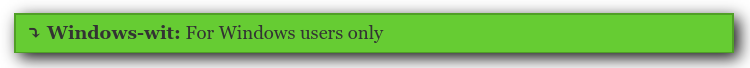
\includegraphics[width=.9\textwidth]{windowswit_web.png}
	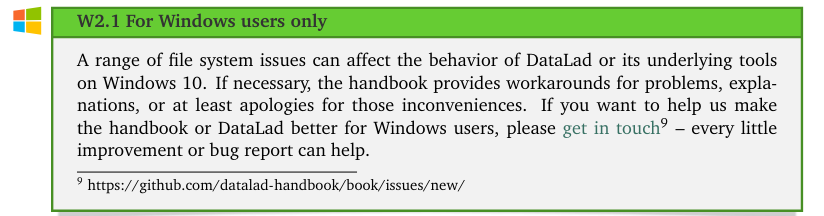
\includegraphics[width=.9\textwidth]{windowswit_pdf.png}
	\caption{Windows-wit}
	\label{fig:handbook-windowswit}
	\end{subfigure}
	\begin{subfigure}{.55\textwidth}
		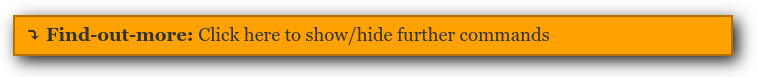
\includegraphics[width=\textwidth]{findoutmore_web.png}
		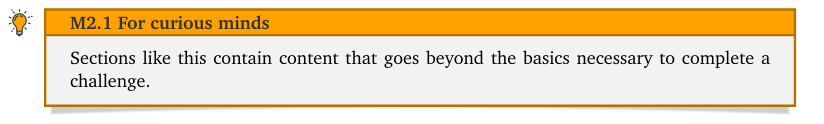
\includegraphics[width=\textwidth]{findoutmore_pdf.png}
		\caption{Find-out-more}
		\label{fig:handbook-findoutmore}
	\end{subfigure}
	\hfill
	\begin{subfigure}{.44\textwidth}
	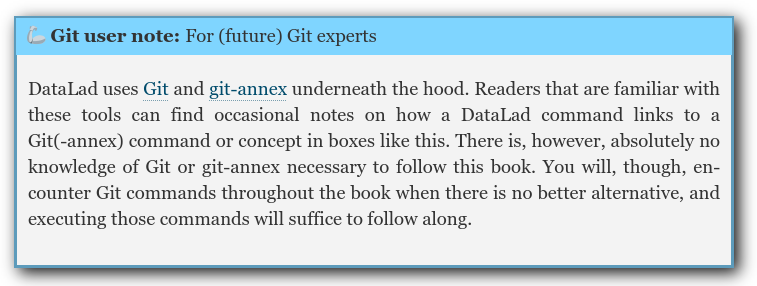
\includegraphics[width=\textwidth]{gitusernote_web.png}
	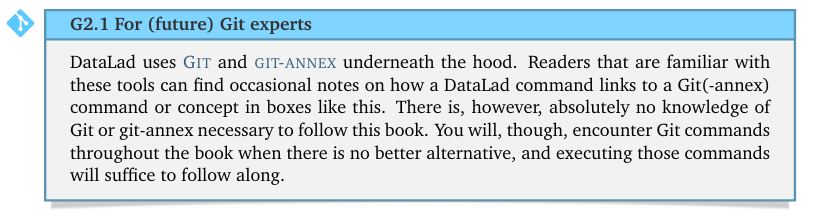
\includegraphics[width=\textwidth]{gitusernote_pdf.png}
	\caption{Git user note}
	\label{fig:handbook-gitusernote}
	\end{subfigure}
	\hfill
	\begin{subfigure}{.55\textwidth}
	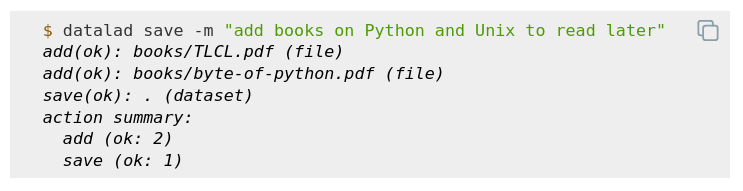
\includegraphics[width=.9\textwidth]{codeblock_web.png}
	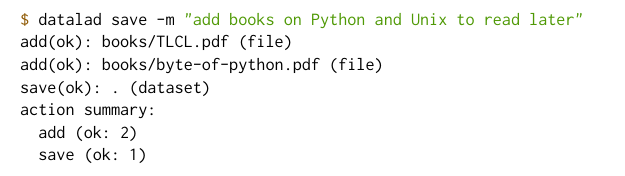
\includegraphics[width=.9\textwidth]{codeblock_pdf.png}
	\caption{Code block}
	\label{fig:handbook-codeblock}
    \end{subfigure}
	\caption[Customization in the DataLad Handbook]{Custom admonitions and code blocks used in the DataLad Handbook. In each panel, the top image corresponds to the web version of the admonition, and the bottom image corresponds to its PDF rendering.
	\ref{fig:handbook-windowswit}: Windows-wits, toggle-able in the HTML version, contain information that is only relevant for the Windows operating system. \ref{fig:handbook-findoutmore}: Find-out-more admonitions, also toggle-able in the HTML version, contain miscellaneous extra information for curious readers. \ref{fig:handbook-gitusernote}: Git user notes are colored boxes with references to the underlying tools of DataLad, intended for advanced Git users as a comparison or technical explanation.  \ref{fig:handbook-codeblock}: Code blocks show one or more commands and the resulting output, provided using the \texttt{autorunrecord} Sphinx extension. In the web version, a copy-button (top right corner) allows to copy relevant commands automatically to the clipboard. Internal annotations allow generating custom scripts from any sequence on code-blocks for live coding demonstrations}
	\label{fig:handbook-admonitions}
\end{figure}

\subsubsection{Content}

The introduction part of the Handbook has two different target audiences:
For one, it provides \textit{researchers} with detailed installation instructions, a basic general command line tutorial, and an overview of the handbook.
Beyond this, it gives a high-level overview of the software and its capabilities to \textit{planners}. \\
The Basics part is organized into 9 chapters.
Following a narrative about a fictional college course on \gls{rdm}, it teaches different aspects of DataLad functionality and general research data management to \textit{researchers} in each topical chapter.
Broadly, those topics can be summarized as follows: 1) Local version control, 2) Capturing and re-executing process provenance, 3) Data integrity, 4) Collaboration and distributed version control, 5) Configuration, 6) Reproducible data analysis, 7) Computationally reproducible data analysis, 8) Data publication, and 9) Error management.
The Beyond Basics part adds independent chapters on advanced DataLad features and workflows, big data projects, DataLad use on computational clusters, DataLad's internals, and selected DataLad extensions.
The latter two parts are accompanied with code demonstrations, slides, executable notebooks, or video tutorials that \textit{trainers} can reuse freely.
The last part, Usecases, targets \textit{planners} and \textit{researchers} with short step by step instructions.
They show planners what is possible, and help researchers connect their knowledge into larger workflows.
% outline the content, with a focus on how they improve scientific practice

\subsubsection{Project and community management}

Ensuring the longevity of software projects beyond the duration of individual researcher's contracts requires community building \citep{koehler2020better}.
A user-driven alternative to documentation by software developers, ``Documentation Crowdsourcing'', has been successfully employed by the NumPy project \citep{pawlik2014crowdsourcing}.
% maybe mention pandas documentation sprint: https://python-sprints.github.io/pandas/
The Handbook project extends this concept beyond reference documentation.
To achieve this, it is set up to encourage and welcome improvements by external contributors.
The project is openly hosted on GitHub.
Mirroring processes in larger crowd-sourced documentation projects such as the ``The Turing Way handbook for reproducible, ethical and collaborative research'' \citep{the_turing_way_community_2022_7625728}, credit is given for both code-based and non-code-based contributions.
Contributors are recognized in the source repository, on the DataLad Website, and as co-authors in both the printed version of the Handbook and its Zenodo releases.
As of TODO-May 2023, a total of TODO-54 contributors provided input in the form of content, bug fixes, or infrastructure improvements.


\subsubsection{Impact and scope}

Work on the DataLad Handbook began in June 2019, and the first release followed in January 2020.
It has been under continuous development for more than four years, averaging two releases per year, and complements  the DataLad ecosystem with a comprehensive user guide.
Releases of the DataLad core package are coordinated with matching releases of the Handbook project, and past release versions remain accessible online.

\begin{figure}
	\begin{subfigure}{.48\textwidth}
		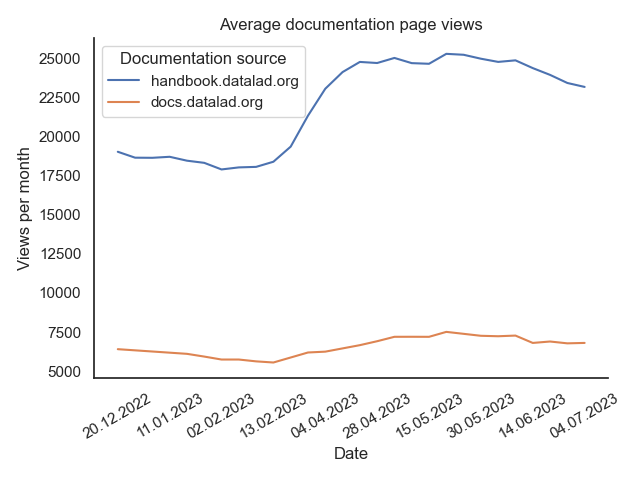
\includegraphics[width=\textwidth]{rtd.png}
		\caption{Monthly documentation views}
		\label{fig:rtd}
	\end{subfigure}
    \begin{subfigure}{.48\textwidth}
	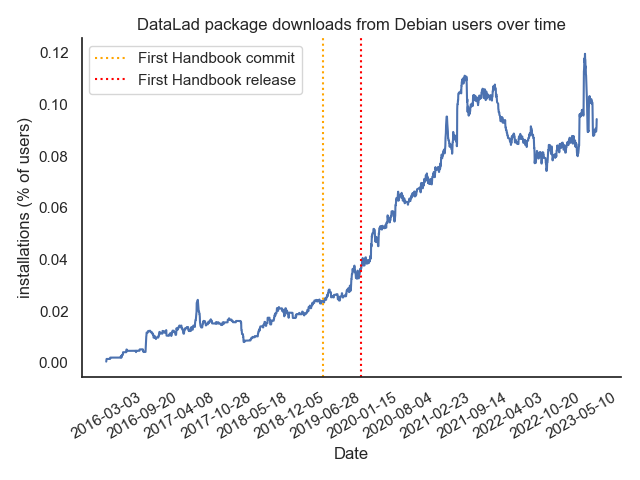
\includegraphics[width=\textwidth]{popcon.png}
	\caption{Debian package popularity counts for DataLad}
	\label{fig:popcon}
	\end{subfigure}
	\caption[Software and documentation popularity]{Software and documentation popularity measures. \ref{fig:rtd}: Documentation page views for the technical documentation (\url{docs.datalad.org}) and the user documentation (\url{handbook.datalad.org}), displayed as average views per 30 days, between December 2022 and May 2023. The DataLad Handbook consistently sees higher traffic.
	\ref{fig:popcon}: Popularity of the Debian packages DataLad and python3-datalad over time, expressed in percent of Debian users that installed the package from the total amount of users submitting download statistics. Dashed lines indicate the fist commit and the first release of the Handbook, the latter marks a notable increase in software downloads. Source: Debian Popularity Contest, May 2024. }
	\label{fig:popularity}
\end{figure}

The web and PDF versions are organized into 4 parts, with a total of 21 chapters across the parts Introduction, Basics, and Advanced, and 12 use cases.
Its PDF version spans more than 600 pages.
An analysis of traffic during from December 2022 and TODO-July 2023 revealed that handbook.datalad.org averaged TODO-2xxxx total page views per 30 days.
In the same time span, the technical documentation of DataLad at docs.datalad.org averaged 7xxxx total page views per 30 days, roughly a third of the traffic of the user documentation (\cref{fig:rtd})


%It has amassed a quarter of the total number of GitHub stars of the DataLad core source repository.

%maybe citations? maybe analyze github stars
Confirming observations from the literature \citep{loggemDDD}, the conjunct development of user-documentation has positive effects on software quality.
As the writing process involves manual software testing, we observed a higher discovery rate of software errors.
The user-focused approach uncovers deficiencies of the technical documentation and \gls{api} elements with suboptimal user experience.
The workflow-based nature of demonstrations highlights API inconsistencies.
And the integration test that the handbook constitutes catches incompatibilities between the software and common usage practice.
% maybe lower barrier of access for non-technical people to raise issues or feature requests
These documentation features facilitate software development, and had a major impact on the conjoint 0.12.0 release of DataLad (Jan 2020), the first with a matching handbook release.
The popularity data in \cref{fig:popcon} confirms a marked increase in downloads from this date onward.

In summary, the development of the DataLad Handbook had a measurable positive impact on the number of users, the popularity of the package, and the software quality.
The project documents workflows that improve scientific practice, such as local and distributed version control, collaboration, data publication, and reproducible analysis.
The next chapter will focus particularly on why these abilities are useful in science, and how they enable trustworthy science at the largest scale.


\pagebreak

